\documentclass[12pt,a4paper]{article}
\usepackage{longtable}
\usepackage[LGR,T1]{fontenc}
\usepackage{lscape}
%\usepackage{pdfsync}
\usepackage{multirow}
\usepackage{amsmath,bm} 
\usepackage{amsfonts}
\usepackage{amsthm} % Extended theorem environments
%\usepackage{amssymb} % Math symbols %%redundant with stix package
%\usepackage{esint} % Intégrales multiples
%\usepackage{esvect} % Vecteurs
\usepackage{mathtools}
\usepackage{pifont} 
 
\usepackage{fancyhdr}
\usepackage{graphicx}

\graphicspath{{../frontend/img/}{../chap_intro_ccl/img/}{../chap_case_study/img/}{../chap_ES_PCE/img/}{../chap_electro_uq/img/}{../chap_methodo/img/}{../chap_myopic/img/}{../chap_RL/img/}{../chap_atom_mol/img/}{../chap_RobPol/img/}{../appendices/img/}} % Figures folder different for each input
%\graphicspath{{img/}} %
\DeclareGraphicsExtensions{.eps,.pdf,.png,.jpg}




\usepackage{lastpage}
\usepackage{afterpage}
\usepackage{lettrine}
\usepackage{color,soul}
\usepackage[dvipsnames]{xcolor}
\usepackage{colortbl}
\usepackage{enumitem}
\usepackage{tikz}
\usepackage{titlesec}
\def\eg{e.g.,\ }
\def\ie{i.e.,\ }


%Palatino font
%\usepackage{pxfonts}
%\usepackage{libertine}
\usepackage[scaled=0.88]{beraserif}
\usepackage[scaled=0.85]{berasans}
\usepackage[scaled=0.84]{beramono}
\usepackage{mathpazo}
%\linespread{1.05}
\usepackage[T1,small,euler-digits]{eulervm}

\usepackage[nomessages]{fp}


\definecolor{bleuUCLclair}{rgb}{.09, 0.569, 1}
\definecolor{bleuUCLfonce}{rgb}{ .13, .52, .86}
\definecolor{redBurn}{rgb}{.91, 0.29, 0.08}

\usepackage{tocloft}
\renewcommand{\cftsecpresnum}{Reviewer \#}
\renewcommand{\cftsecnumwidth}{6em}
\renewcommand{\cftsubsecpresnum}{Comment \#}
\renewcommand{\cftsubsecnumwidth}{6em}

\usepackage[colorlinks=true,urlcolor=black,linkcolor=black,citecolor=black]{hyperref}
\usepackage[square,numbers,sort&compress]{natbib}

\bibliographystyle{biblio/elsarticle-num-names}  %Ordered by appearance in the text, with DOI and URL
%\usepackage[backend=biber, natbib=true, style=numeric-comp, citestyle=numeric-comp, sorting=none, giveninits=true, maxcitenames=1]{biblatex}

\usepackage[]{tocbibind}
\usepackage{hyperref}
\hypersetup{
    colorlinks=true,
%    linkcolor=black,
    bookmarks=true,
    pdfpagemode=FullScreen,
}
\setcounter{tocdepth}{1}

\addtolength{\topmargin}{-1.5cm}
\addtolength{\textheight}{1.5cm}
\addtolength{\textwidth}{2cm}
\addtolength{\footskip}{2cm}
\setlength{\evensidemargin}{-0.5cm}
\setlength{\oddsidemargin}{-0.5cm}
\setlength{\arrayrulewidth}{0.25pt}

\renewcommand{\baselinestretch}{1.1} % Interligne


\newenvironment{maliste}%
{ \begin{list}%
	{\textcolor{bleuUCLfonce}{$\bullet$}\hspace{0.5cm}}%
	{\setlength{\labelwidth}{50pt}%
	 \setlength{\leftmargin}{25pt}%
	 \setlength{\itemsep}{30pt}}}%
{ \end{list} }

%\renewcommand{\headrulewidth}{0.0pt}
%\newcommand{\clearemptydoublepage}{%
%	\newpage{\pagestyle{empty}\cleardoublepage}}




%section like title in longtable
\newcommand{\seclong}[1]{\multicolumn{2}{@{}l}{{\Large\sffamily #1}} 
\vspace{0.5cm}
\\}

%enumerate on two columns
\newcounter{listlong}
\newcommand{\newlistlong}{\setcounter{listlong}{1}}
\newcommand{\iteml}[1]{%
\hspace{4.5cm}\textcolor{redBurn}{\arabic{listlong}}\stepcounter{listlong}%
&%
#1%
 
\\%
}

%left in column
\newcommand{\lcol}[1]{%
\begin{minipage}[t]{.35\textwidth}%

#1%

\end{minipage}%
}

\title{\vspace{-1cm}
\begin{flushleft} {\sffamily Xavier Rixhon's PhD thesis - Answers to jury members}\end{flushleft}}
\date{\vspace{-1.7cm}\begin{flushleft}\sffamily Exploration of uncertainty-aware energy transition pathways - Reinforcement learning and principal component analysis-based methods\end{flushleft}}
%
%Xavier Rixhon, Gauthier Limpens, Diederik Coppitters, Hervé Jeanmart and Francesco Contino\end{flushleft}}


\pagestyle{fancy} 
\fancyhf{}
\fancyfoot[R]{\sffamily\thepage\ / \pageref{LastPage}}
  \fancyfoot[L]{ }

\fancypagestyle{plain}{%
  \fancyhf{}%
  \fancyfoot[R]{\sffamily\thepage\ / \pageref{LastPage}}
  \fancyfoot[L]{ }
}

\renewcommand{\headrulewidth}{0.0pt}


\newcommand{\hlc}[2][yellow]{ {\sethlcolor{#1} \hl{#2}} }

\titleformat{\section}
  {\bfseries\scshape}{}{1em}{}

\titleformat{\subsection}
  {\normalfont\scshape}{}{1em}{}

\usepackage[framemethod=default]{mdframed}
%\mdfsetup{skipabove=\topskip,skipbelow=\topskip}

\global\mdfdefinestyle{comment}{%
     linecolor=red,linewidth=0.1cm,%
     leftmargin=-0.5cm,rightmargin=-0.5cm, innerleftmargin=0.4cm,innerrightmargin=0.4cm,
     topline=false,bottomline=false
}

\global\mdfdefinestyle{manuscript}{%
     linecolor=gray!20,linewidth=0.05cm,backgroundcolor=gray!20,%
     leftmargin=-0.5cm,rightmargin=-0.5cm, innerleftmargin=0.4cm,innerrightmargin=0.4cm
}
  
  \renewcommand{\subsectionautorefname}{Comment}
\begin{document}
\maketitle
%\emph{Start with some thank you note. For example:}

I would like to thank the jury members for the comments, which significantly helped improving the manuscript and substantiating the novelty of my work. Based on the notes taken during the private defense, I hereby transcribed, as accurately as possible, the jury's comments. 

I believe I have addressed all the issues raised in the following answers. Some of them required adaptations of the text. These adaptations are either directly in the thesis manuscript or left for further developments in subsequent papers. For each comment, I have first highlighted the issue, then provided an answer, and finally described how the manuscript was adjusted, if needed.\\

When a comment explicitly came from specific members of the jury, they are listed at the beginning of the comment with the following color code: {\color{orange} \textbf{Stefano} Moret}, {\color{teal} \textbf{Stefan} Pfenninger}, {\color{purple} \textbf{Sylvain} Quoilin} and {\color{violet} \textbf{Christophe} De Vleeschouwer}. Here is how an answer to a comment is structured:

\begin{mdframed}[style=comment] % Comment from the reviewer
Text of the comment.
\end{mdframed}

\noindent The answer provided to the comment and, based on this, where the potential modification brought to the manuscript is located in the thesis manuscript using {\color{blue} blue font}.

\begin{mdframed}[style=manuscript] % Modification brought to the manuscript
New version of the text in the manuscript.
\end{mdframed}

\clearpage

%
% Reviewer 1
%
\section{Introduction}
\label{Introduction}
%Thank you for the reviews and comments to the manuscript we submitted to the Frontiers Journal. In the following, we carefully addressed each point raised by Reviewer 1, and revised the main manuscript and the supporting information accordingly. The following replies include as well all the changes we made to our manuscript based on your comments.

\subsection{Literature review}
\label{Intro_lit_review}



\section{Reinforcement Learning}
\label{RL}
%Thank you for the reviews and comments to the manuscript we submitted to the Frontiers Journal. In the following, we carefully addressed each point raised by Reviewer 1, and revised the main manuscript and the supporting information accordingly. The following replies include as well all the changes we made to our manuscript based on your comments.

\subsection{Binding}
\label{RL_binding}

\begin{mdframed}[style=comment] % Comment from the reviewer
{\color{violet} \textbf{Christophe}} - The concept of binding constraint was not clear.
\end{mdframed}

\noindent
Besides the information given in Section 4.2.3 of the manuscript (and reminded here below), I do not see further explanations that could clarify the concept of binding constraint in a Linear Programming (LP) problem. Consequently, regarding this comment, there has not been further modification brought to the manuscript.


\begin{mdframed}[style=manuscript] % Modification brought to the manuscript
To identify the actions that have an actual impact on the environment, we can check if they are binding or not. In a LP problem, constraints represent hyperplanes in the domain of variables. In a two-dimension space, these are straight lines (see Figure \ref{fig:Binding_constr}). When the problem is bounded and feasible, these lines are the edges of a convex polygon: the domain of feasibility. The optimal solution, $\textbf{x}^*$, is the combination of variables leading to the optimal value of the objective function. Besides being within the domain of feasibility, it is proven that this optimal solution, when unique\footnote{There are cases where the objective function has the same optimal value along an entire edge. In this case, there is an infinity of solutions and the problem is indeterminate.}, locates on a vertex of the domain \cite{bertsimas1997introduction}. The constraints intersecting at this vertex are considered as binding, actually limiting the objective function to be more optimal. In other words, binding constraints, when tightened, aggravate the objective value function. If these are inequality constraints, as represented in Figure \ref{fig:Binding_constr}, it means that their left and right sides of the equation are equal.
\end{mdframed}

\begin{figure}[!htbp]
\centering
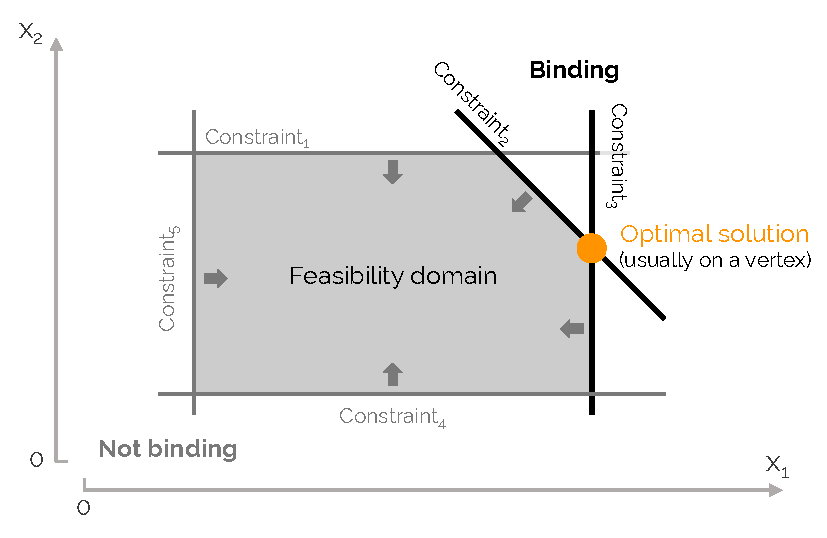
\includegraphics[width=0.7\textwidth]{Binding_constr.pdf}
\caption{Binding versus non-binding constraints. In LP where the feasibility domain is non-empty and bounded, the constraints defined a convex feasibility domain in the space of variables (here, x$_1$ and x$_2$). The optimal solution usually locates on a vertex of this domain, \ie the intersection of several constraints (here, constraints 2 and 3) limiting the solution. These constraints are considered as binding, \ie having a limiting impact on the optimal solution.}
\label{fig:Binding_constr}
\end{figure}

\section{Principal Component Analysis}
\label{PCA}

\subsection{Confusion with the word PC}
\label{Confusion_PC_wording}


\begin{mdframed}[style=comment] % Comment from the reviewer
{\color{violet} \textbf{Christophe}} When using the word ``component'', there seems to be a confusion and it is not always easy to understand if you refer to the vector or the coefficient related to one of the original variable.
\end{mdframed}

\noindent The confusion probably comes from the fact a Principal Component (PC) actually represents an eigenvector of the covariance matrix. This vector is, by definition, composed of \textbf{components}, each of them being a coefficient related to a specific original variable. Here below the parts where there could have been misleading confusion are listed and, potentially, modifications have been brought to the manuscript:

{\color{blue} End of second paragraph of section 1.4.1 - no modification}:

\begin{mdframed}[style=manuscript] % Modification brought to the manuscript
Moreover, this means that $\alpha_{ki}$, \ie the \textbf{component} of $\bm{\alpha}_{\mathbf{k}}$ related to the $i^{\text{th}}$ original variable, $x_i$,  gives its weight in the $k^{\text{th}}$ PC, \ie $z_k$. 
\end{mdframed}


\clearpage
\def\bibfont{\scriptsize}
\bibliography{../bib_thesis.bib}
\normalsize

\end{document}